\documentclass[]{article}
\usepackage[a4paper, total={5in,10in}]{geometry}
\usepackage{hyperref}
\usepackage{siunitx}
\usepackage[backend=biber]{biblatex}
\addbibresource{report.bib}
\usepackage{graphicx}
\usepackage{caption}

%opening
\title{EP2420 - Project 1: Task II - 2.2, Task III}
\author{André Silva}
\begin{document}

\maketitle

\section{\textbf{Task II - 2.2}}
\label{sec:1}

\begin{figure}[h!]
    \centering
    \captionsetup{justification=centering}
    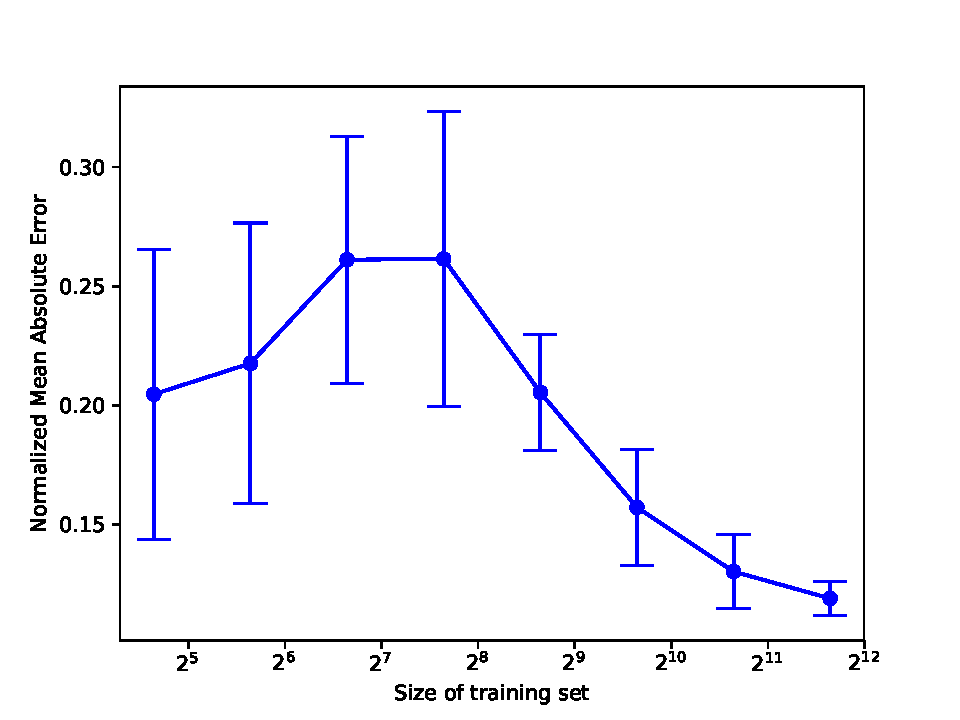
\includegraphics[width=0.75\textwidth,height=\textheight,keepaspectratio]{../result/project1/training_set_size_errors.pdf}
    \caption{Measured \textit{Normalized Mean Absolute Error} for a given training set size using \textit{Lasso Regression}~\cite{Lasso}. Error bars represent $2\sigma$ over 50 measurements. Data points represent means.}
    \label{fig:1}
\end{figure}

Intuition tells us that the more information we have access to, the better conclusion we can extract from them.

By looking at (\ref{fig:1}), we notice that the curve begins by unexpectedly increasing, followed by an expected decrease. 

We can also notice that the variance of the measurements starts off very high, and shows a decreasing tendency as we increase the size of the training set. This partly explains why the curve doesn't follow our initial expectations. 

Another reason that can explain this is the fact that outliers in small training sets have a higher influence than in large training sets, and the probability of including outliers in randomly picked training sets decreases as we decrease its size.

Overall, we can conclude that the larger a training set is the better a model can predict the system, as the training set becomes more general and so more information can be inferred from it.

\pagebreak

\section{\textbf{Task III}}
\label{sec:2}

\begin{figure}[h!]
    \centering
    \captionsetup{justification=centering}
    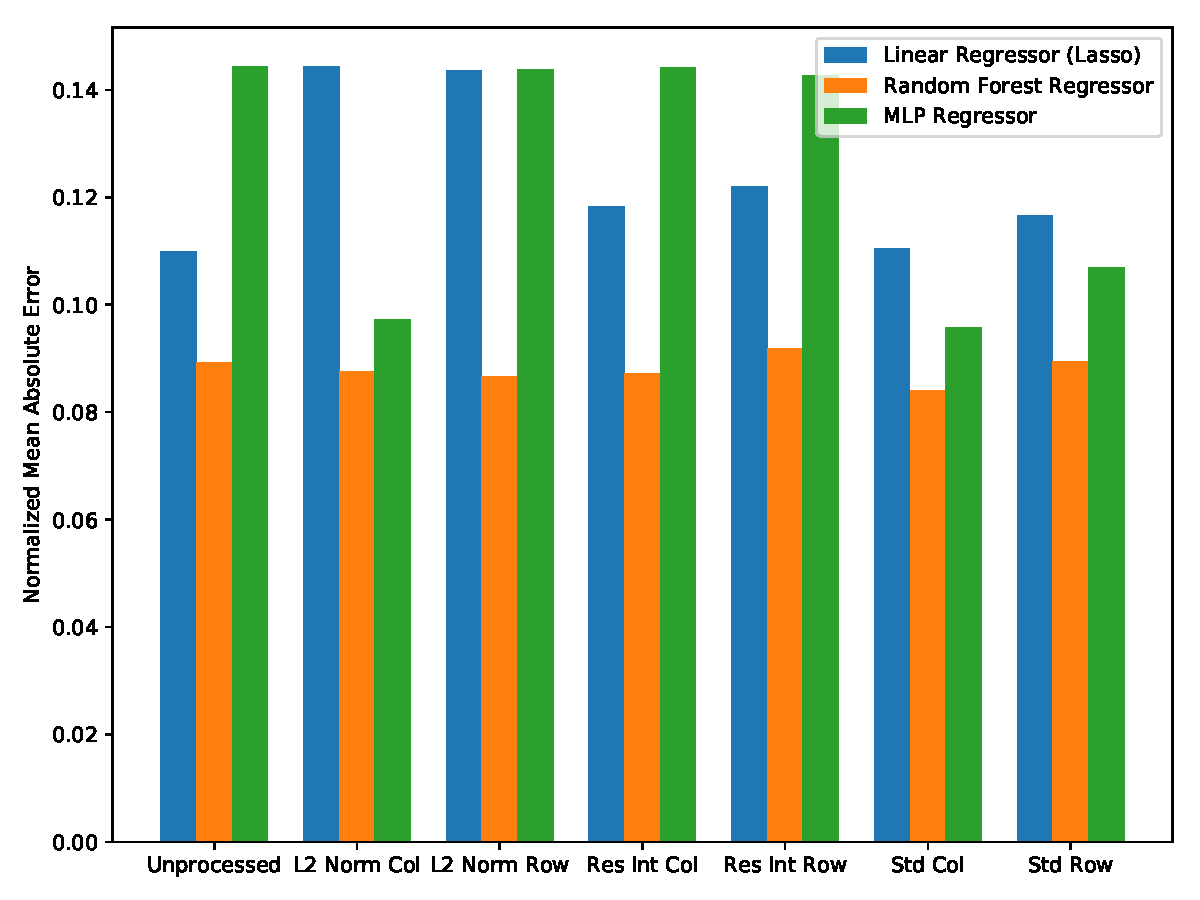
\includegraphics[width=0.72\textwidth,height=\textheight,keepaspectratio]{../result/project1/pre_processing_accuracies.pdf}
    \caption{Measured \textit{Normalized Mean Absolute Error} for a given pre-processed dataset.}
    \label{fig:2}
\end{figure}

In (\ref{fig:2}), we can see that pre-processing the data impacts some models more than others.

In the case of \textit{Random Forest Regression}~\cite{RFR}, the gains or losses of accuracy are marginal for all pre-processing methods. This happens by definition, since tree partition algorithms are not affected by the scaling or centralization of datapoints.

\textit{MLP Regressor}~\cite{MLPR} seems to be the model which suffers the biggest impact from data pre-processing, showing either no difference or a considerable gain.

\textit{Lasso}~\cite{Lasso} consistently shows worse performance on pre-processed data when compared to the original one.

By analyzing (\ref{fig:2}) again, we can see that standardizing along each column is the method that results in the best results for all 3 regression techniques.

\begin{figure}[h!]
    \centering
    \captionsetup{justification=centering}
    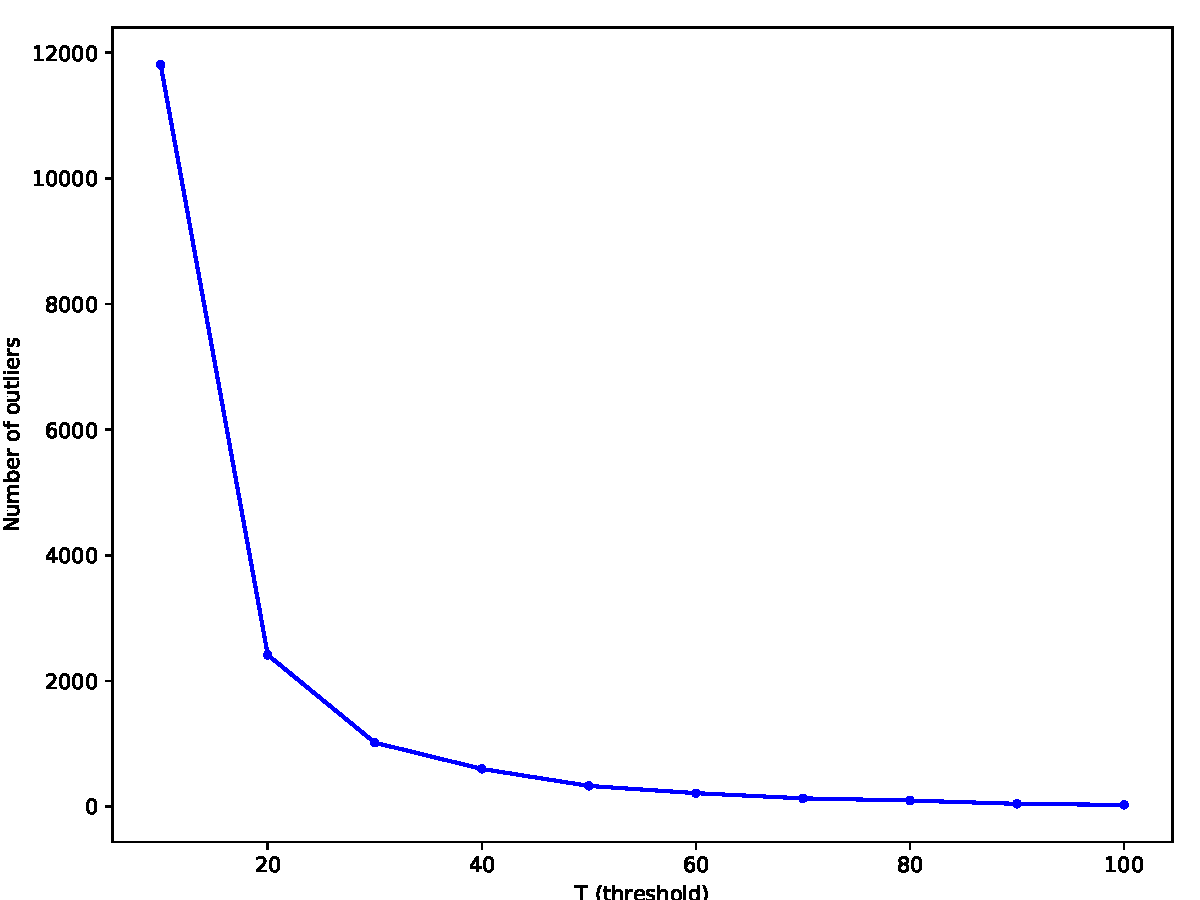
\includegraphics[width=0.72\textwidth,height=\textheight,keepaspectratio]{../result/project1/number_outliers.pdf}
    \caption{Number of outlier points for a given threshold on the standardized design matrix along each column.}
    \label{fig:3}
\end{figure}

(\ref{fig:3}) shows, as expected, a function that decreases while T increases, eventually converging to 0. This happens because we have standardized the data along each column, making each feature space look like a Gaussian distribution with 0 mean and unit variance.

As we filter rows based on absolute values, we will find less and less examples of outliers as T increases, by the definition of a Gaussian distribution.

\pagebreak

\begin{figure}[h!]
    \centering
    \captionsetup{justification=centering}
    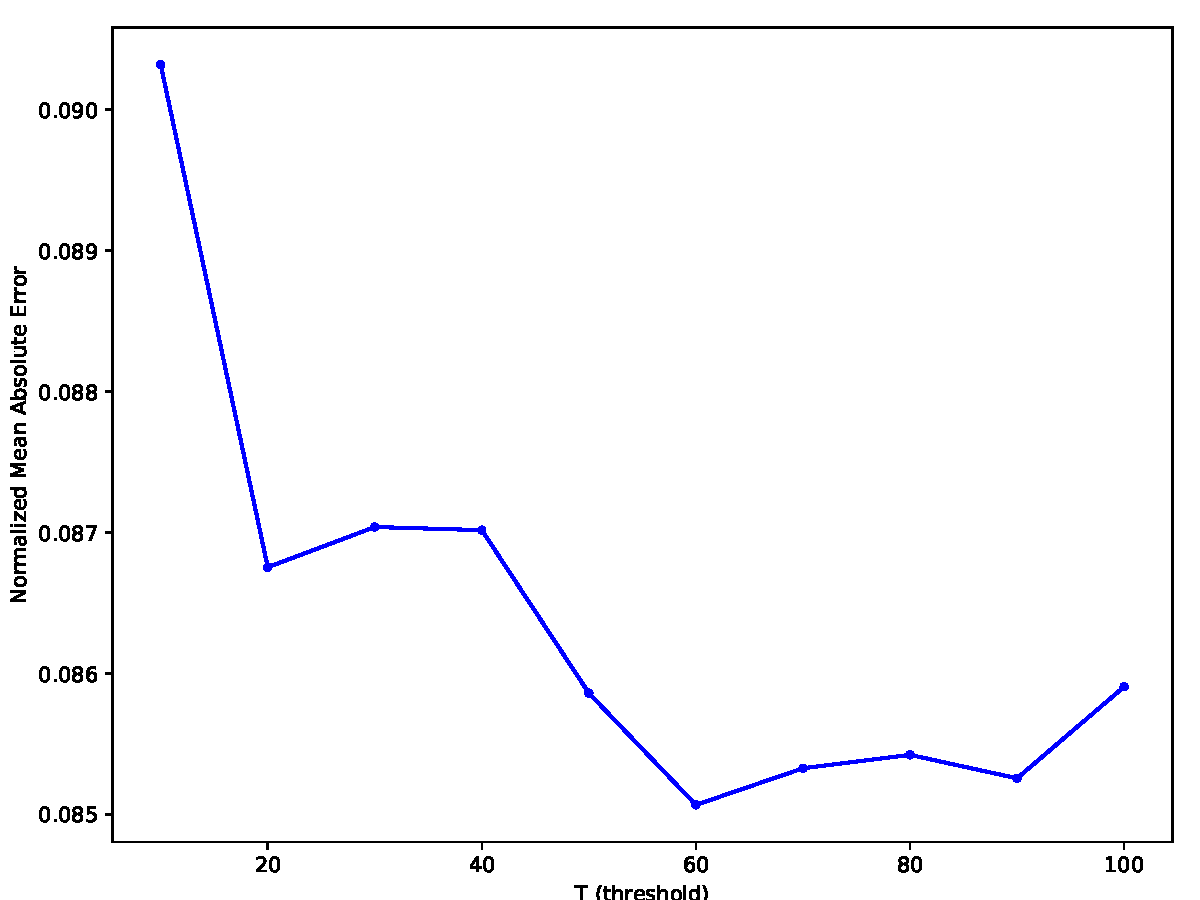
\includegraphics[width=0.75\textwidth,height=\textheight,keepaspectratio]{../result/project1/nmae_outliers.pdf}
    \caption{\textit{Normalized Mean Absolute Error} for a given threshold T (outlier removal) using \textit{Random Forest Regression}~\cite{RFR}.}
    \label{fig:4}
\end{figure}

(\ref{fig:4}) shows us that the \textit{NMAE} starts off by decreasing, as we increase the threshold for outlier removal, suggesting low threshold values may lead to the removal of important parts of the dataset. As we incorporate more datapoints in our dataset, we can better predict outcomes. This goes in hand with the results of section (\ref{sec:1}).

As we reach a very high treshold we notice a slight increase, which might represent the impact more extreme outliers have on the outcome of the tested model, \textit{Random Forest Regression}~\cite{RFR}. This approximation to a parabola was the expected result for this experiment.

\printbibliography

\end{document}
